% $Id: firststeps.tex 6498 2008-02-13 10:43:03Z alexandra $
% Local Variables:
% ispell-check-comments: nil
% Local IspellDict: american
% End:
% --------------------------------------------------------
% User documentation
% copyright by BREDEX GmbH 2004
% --------------------------------------------------------
%% This section provides a basic working example for \GD{}.
%% A simple \bxname{Java} program (\bxname{Adder})
%%  has been provided to serve as an \gdaut{}.
%% This program will be tested by entering several numbers 
%% to be added and checking the results. There is, however,  a deliberate
%% error in the program;
%%  the values 17 and 4 give \bxcaption{jackpot} as the result. 
%% In this way, the results will show both successful and failed \gdcases{}.  

%% The views and editors referred to during this example can be
%%  seen in \bxfigref{clientwindow}.
%% \subsubsection{Creating and Configuring the \gdproject}
%% \begin{enumerate}
%% \item Select:\\ \bxmenu{Project}{New}{} and enter the username and password for
%% the \gddb when prompted.

%% Use the username \bxshell{sa} and leave the password field blank to use
%% the default \gddb{}. Otherwise, enter the details for an 
%% individual user \gddb{}. 

%% \item In the \gdproject dialog, enter \bxshell{SimpleAdder}
%%  as the  \gdproject name, choose \bxcaption{English (United States)} as the 
%% \gdproject language and select \bxcaption{Next}.

%% \item Enter \bxshell{Adder} as the \gdaut name, choose \bxcaption{English}
%% as the \gdaut language and select \bxcaption{Next}.

%% \begin{figure}[h]
%% \begin{center}
%% %\includegraphics[width=\bxpicwidth]{GettingStarted/PS/AUTconfig}
%% \includegraphics[width=12cm]{GettingStarted/PS/AUTconfig}
%% \caption{\gdaut configuration window}
%% \label{AUTconfig}
%% \end{center}
%% \end{figure}


%% \item Enter \bxshell{Adder configuration} as the \gdaut configuration name 
%% (see \bxfigref{AUTconfig}).
%% \item Choose the server  (e.g. \bxcaption{localhost}) or add a new one.
%% \item Enter the JAR file name, 
%% (i.e. \bxshell{C:$\backslash$Program Files$\backslash$GUIdancer$\backslash$aut$\backslash$adder$\backslash$adder.jar}).
%% \item If the \gdaut needs to be activated before testing can begin, select the checkbox to activate the \gdaut and choose an activation method from the combo box. 
%% \item The \bxname{Java} runtime location may also be defined, either by choosing one 
%% of the available ones from the list, or by adding another. 
%% (e.g 
%% \bxshell{C:$\backslash$Program Files$\backslash$Java$\backslash$jre1.5.0$\backslash$bin}).
%% \item Add any necessary parameters, then select \bxcaption{Next} then \bxcaption{Finish}.
%% \end{enumerate}

Once a project has been created, \gdcases{}, \gdsteps and \gdsuites can be
created within it. 

\subsubsection{Creating a \gdcase}

The following steps will create a \gdcase containing
four \gdsteps which will enter values into the two fields in the 
Adder program, then  calculate and check
the answers.   

\begin{enumerate}
 \item In the \gdtestcasebrowser{} double-click on the \bxcaption{Test Cases:}
 node
and enter \bxshell{First Test} 
when prompted for a name. Select \bxcaption{Ok}.
\item This will produce a \gdcase node in the  \gdtestcasebrowser{}, with the
name just entered. Double-click on this node. 
\item In the editor which appears, double-click on the
 \bxcaption{First Test} node. 
This will produce a dialog to specify a \gdstep{}. 
\begin{itemize}
\item Enter \bxshell{input first value} as the name.
\item Select \bxcaption{Text Field} as the component type.
\item Enter \bxshell{F1} as the component name.
\item Select \bxcaption{Replace Text} as the action.
\item Press \bxcaption{Ok}.
\end{itemize}
\item In the \gdpropview{} in the top right-hand corner of the perspective, double click in the \bxcaption{parameter value} cell and 
 enter \bxshell{=V1} (this is a reference for the number to be  entered in
the field) and press \bxcaption{Save}.
\item Create another
 new \gdstep by double-clicking again on the \bxcaption{First
Test} node in the 
editor. This second 
\gdstep should contain  exactly the same details as the previous,
 only changing the \gdstep name to \bxshell{input second value}, the
component name to \bxshell{F2} and the parameter value to \bxshell{=V2}
\item Create two more \gdsteps as above and name them \bxshell{calculate} and 
\bxshell{verify} respectively. The \gdsteps should be specified as follows:

\begin{itemize} 
\item For the ''calculate'' \gdstep:
\\
\\
\begin{tabular}{|p{0.3\bxpicwidth}|p{0.3\bxpicwidth}|}\hline
 Component type:& Button\\\hline
 Component name:& \bxshell{calculate}\\\hline
 Action:& Click\\\hline
 Parameter -- Number of Clicks:& 1 (Default)\\\hline
Parameter -- Mouse Button:& 1 (Left -- Default) \\\hline
\end{tabular}
\\
\\
\item For the ''verify'' \gdstep{}:
\\
\\
\begin{tabular}{|p{0.3\bxpicwidth}|p{0.3\bxpicwidth}|}\hline
 Component type:& Text Field\\ \hline
 Component Name:& \bxshell{result}\\ \hline
 Action:& Verify text\\ \hline
Parameter:& =RES\\ \hline
\end{tabular}
\end{itemize}

\item Press the \bxcaption{save} button on the toolbar.
\end{enumerate}

  The \gdcase \bxcaption{First Test} should now contain four \gdsteps{}:
\begin{itemize}
\item \bxcaption{input first value}  
\item \bxcaption{input second value}
\item \bxcaption{calculate}
\item \bxcaption{verify}

Behind the name of the  \gdcase in the \gdtestcaseeditor{}, the
 parameters \bxcaption{V1; V2; RES} should be displayed in square brackets 
(\bxfigref{firsttest}). 
\end{itemize}

\begin{figure}[h]
\begin{center}
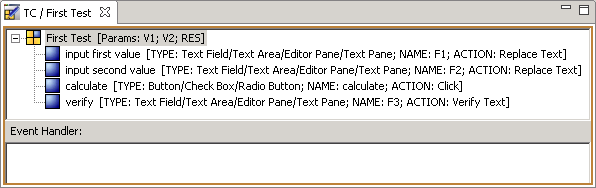
\includegraphics{GettingStarted/PS/firsttesteditor}
\caption{First Test \gdcase}
\label{firsttest}
\end{center}
\end{figure}

If the \gdsteps are in the wrong order, use drag-and-drop to re-order them.

\subsubsection{Adding Test Data}

\begin{enumerate}

\item In the \gdtestcaseeditor{}, single-click on the \bxcaption{First Test}
 node. 
In the Data Sets View in the top right-hand corner of the 
perspective, select \bxcaption{Add} and in the
row which appears, enter \bxshell{3} in the  field for 
\bxcaption{V1}, \bxshell{2} in the field for \bxcaption{V2} and \bxshell{5}
in the field for \bxcaption{RES}. 

\item Select  \bxcaption{Add} again. In the second row which appears, enter:
\\
\\
\begin{tabular}{|p{0.3\bxpicwidth}|p{0.3\bxpicwidth}|}\hline
 V1:& 17\\ \hline
 V2:& 4\\ \hline
 RES:& 21\\ \hline
\end{tabular}

\item Repeat the above step once more for a third row, with the values:
\\
\\
\begin{tabular}{|p{0.3\bxpicwidth}|p{0.3\bxpicwidth}|}\hline
 V1:& 40\\ \hline
 V2:& 2\\ \hline
 RES:& 42\\ \hline
\end{tabular}

\item Press \bxcaption{Save}.
\end{enumerate}

\subsubsection{Creating the \gdsuite}
Once the \gdcase is complete:
\begin{enumerate}
\item Right
 click in the \gdtestsuitebrowser{}, select:\\
\bxmenu{New}{\gdsuite{}}{} and when prompted,
 name it \bxshell{SimpleAdderTest}.
A \gdsuite node will appear with this name in the \gdtestsuitebrowser{}, and 
the \gdsuiteeditor will appear. In the \gdpropview for  this editor,
 \bxcaption{Adder} will be visible as the  \gdaut name and
 \bxcaption{Adder configuration} as the \gdaut configuration.

\item Drag the \gdcase \bxcaption{First Test} from the 
\gdtestcasebrowser to the \gdtestsuiteeditor{} and drop it onto the node for 
\bxcaption{SimpleAdderTest} \gdsuite{}. 
\end{enumerate}

\subsubsection{Connecting to the \gdserver and starting the \gdaut}
The following steps can be carried out at any point during specification, 
 but must be carried out before object mapping, observation or testing begins. 

\begin{enumerate}
\item Press the \bxcaption{Connect to \gdserver} button on the toolbar. The
status of the \gdserver connection will be visible in the status bar in the bottom
right-hand corner. 
\item Press the \bxcaption{Start \gdaut} button on the toolbar. The
\gdaut will appear and the  status 
bar will change to show the new status. Depending on the system 
configuration, the Adder may be hidden behind some other window. Bring the 
Adder to the front to continue. 
\end{enumerate}

\subsubsection{Object mapping}
Object mapping involves two steps: collecting the objects from the 
\gdaut and assigning them to the component names defined by the user. 

\begin{enumerate}
\item To open the \gdomeditor{}, right click on the node for 
\bxcaption{SimpleAdderTest}and select:\\
\bxmenu{Open with}{\GD object mapping editor}{}
\item In the editor which appears, 
right-click and select  \bxcaption{Start object mapping mode} from the 
context-sensitive menu. 
\item Activate the 
\gdaut{} by clicking in its title bar. 

Supported components display a green border when the cursor
is within them.
\item Hover the cursor over the \bxcaption{value1} text input field 
(just left of the \bxcaption{value1} label) and press
\bxkey{Ctrl+Shift+A}. 
\item Repeat this step three times, hovering over the 
\bxcaption{value2} field, the equals sign and the \bxcaption{result} field,
respectively. 

This will collect the names of the objects in the \gdaut{} and
list them under the category \bxcaption{unassigned technical names}.
\item The collected technical 
names can then be mapped to the component names defined
during the creation of \gdsteps{}. The component names are listed under 
\bxcaption{unassigned component names}.  
\item In
 the \gdomeditor{}, select  \bxcaption{Stop object mapping mode} from
 the context-sensitive menu
 and drag and drop \bxcaption{F1} to \bxcaption{value1}, \bxcaption{F2}
 to \bxcaption{value2} 
\bxcaption{calculate} to \bxcaption{equal} and \bxcaption{result} to
 \bxcaption{result}. 
 \item Press \bxcaption{Save}. 
\end{enumerate}

\subsubsection{Test Execution}
In order to be able to see the test being executed, select: \\ 
\bxmenu{Window}{Preferences}{}
 and select the option to minimize \GD while executing a \gdsuite{}.

Press the \bxcaption{Start a \gdsuite}, and select \bxcaption{Yes}
if asked if the perspective should be automatically changed. 
The test will then be carried out.

\bxwarn{Do
 not carry out any other actions while the test is
running unless the \gdserver and client are installed on different machines.}

 Once testing has finished,
the Execution perspective will appear with the results of the test
 (\bxfigref{Testshot}). 

\subsubsection{Accessing the \gdproject}
This example \gdproject can also be imported into the \gddb{}.
To see the \bredex version, select:\\
\bxmenu{Project}{Import}{} and choose to enter a whole \gdproject{}. The 
location to browse to is: 

C:$\backslash$Program Files$\backslash$guidancer$\backslash$aut$\backslash$adder$\backslash$SimpleAdder.xml
\begin{figure}[h]
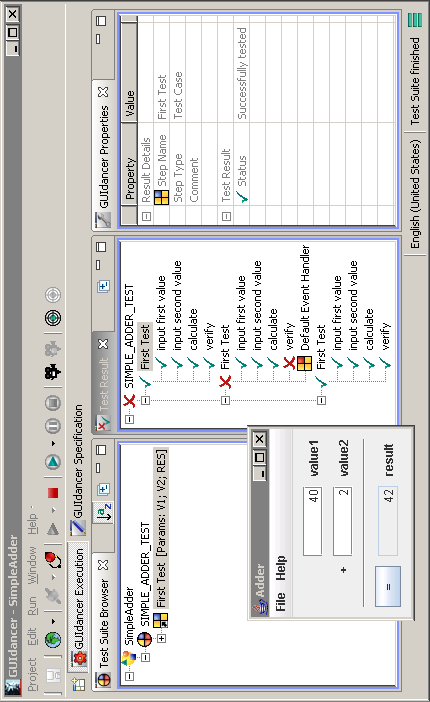
\includegraphics{GettingStarted/PS/Execution}
\caption{Example \gdsuite}
\label{Testshot}
\end{figure}


%The user must then:
%\begin{enumerate}
%\item focus the \gdtestcasebrowser
%\item create a new \gdcase: \bxmenu{New}{\gdcase{}}{}.
%\item select the new \gdcase in the \gdtestcaseeditor 
%\item create a new \gdstep e.g. First start to test the \bxname{DVD-Tool}
%which is included on the installation disk. Try to test the
%\bxmenu{Help}{Info\dots{}}{} menu. 


%Now we will specify  a test which opens the \bxmenu{Help}{Info\dots{}}{} window  
%dialogue and closes it by using the
%\bxcaption{OK}-Button. 
%Two steps are necessary to do this. 
%\end{enumerate}

%There are also two kinds of components with different actions necessary to carry out
%this test.  
%\begin{enumerate}
%\item open \bxmenu{Help}{Info\dots}{} 
%\item click the \bxcaption{OK}-Button
%\end{enumerate}
